\documentclass[11pt]{article}
\usepackage[a4paper,margin=1in]{geometry}
\usepackage{amsmath,amssymb,amsthm}
\usepackage{booktabs}
\usepackage{graphicx}
\usepackage[authoryear,round]{natbib}
\usepackage[hidelinks]{hyperref}
\usepackage{setspace}
\usepackage{caption}
\usepackage{threeparttable}
\usepackage{mathpazo}
\usepackage[T1]{fontenc}
\captionsetup{font=small,labelfont=bf}
\setstretch{1.25}
\newtheorem{proposition}{Proposition}
\newcommand{\R}{\mathbb{R}}
\newcommand{\E}{\mathbb{E}}

\title{Does Wasserstein Robustness Rescue Machine-Learning Portfolios?\\[4pt]
\large Regime Uncertainty, Adaptive Ambiguity and Trading Costs:\\ Evidence from 41 Years of Out-of-Sample Industry Returns}
\author{Muhammad Usama Rashid Malik\thanks{University of Exeter. Email: \href{mailto:usamarm68@gmail.com}{usamarm68@gmail.com}. Replication code is available from the author on request. All errors are my own.}}
\date{Working paper --- This version: September 2026}

\begin{document}
\maketitle

\begin{abstract}
\noindent
I ask whether Wasserstein distributionally robust optimisation (W-DRO) turns machine-learning (ML) return forecasts into better portfolios once trading costs, realistic constraints and regime shifts are taken seriously. Using the 49 Fama--French industry portfolios and 492 months of strictly out-of-sample returns (July 1985 to June 2026), I embed Lasso, random-forest and gradient-boosting forecasts in plug-in, ridge-penalised and W-DRO mean--variance portfolios under identical constraints, with every robustness parameter chosen by rolling validation. Three findings emerge. First, robustness does not create performance: across three forecasters and eight radii, W-DRO moves the net Sharpe ratio by at most 0.07 relative to the plug-in portfolio (under 0.02 for the tree-based forecasts), none of the tested differences is significant, and no forecast-based portfolio beats a forecast-free minimum-variance portfolio; at 50 basis points of trading cost the tree-based strategies underperform it significantly. Second, what robustness does buy is implementability: large radii cut turnover by up to 75\% with no measurable loss of Sharpe ratio. I show that the widely used mean-only W-DRO portfolio is exactly a ridge-penalised portfolio, and the two are empirically indistinguishable; the full Wasserstein mean--variance formulation of \citet{blanchet2022} delivers modestly lower turnover than ridge at equal Sharpe ratio. Third, regime uncertainty, measured by the entropy of filtered hidden-Markov regime probabilities, predicts when tree-based forecasts lose their cross-sectional ranking ability, and market volatility does not explain this. Yet scaling the Wasserstein radius by regime entropy fails to improve portfolios. The evidence cautions against reading simulated or hindsight-tuned DRO gains as proof that robustness extracts value from weak forecasts.

\medskip
\noindent\textbf{Keywords:} portfolio optimisation; distributionally robust optimisation; Wasserstein distance; machine learning; regime switching; transaction costs; out-of-sample evaluation

\noindent\textbf{JEL classification:} G11, C44, C58, C61
\end{abstract}

\newpage
\section{Introduction}

Machine-learning methods predict stock returns better than linear benchmarks in large cross-sections \citep{gu2020}, and a natural next step is to feed those forecasts into a portfolio optimiser. The step is hazardous. Mean--variance optimisers magnify estimation error \citep{michaud1989}, and a long literature finds that simple rules such as equal weighting are hard to beat once estimation error and trading costs are counted \citep{demiguel2009rfs}. ML forecasts make the problem sharper, not easier: they are noisy, their error distribution is unknown and it may shift when the market changes regime.

Distributionally robust optimisation offers an appealing response. Instead of trusting one estimated return distribution, the investor optimises against the worst distribution within a Wasserstein ball around it \citep{esfahani2018,kuhn2019}. The radius of the ball is a dial between trusting the forecast and ignoring it. This paper asks a direct empirical question: \emph{on real data, with identical constraints for every strategy and with the dial set without hindsight, does Wasserstein robustness make ML-driven portfolios better?} I also ask whether the dial should move with the market: if forecasts fail mainly when the regime is uncertain, the radius should widen exactly then.

To answer these questions I run a horse race on the 49 Fama--French industry portfolios from July 1985 to June 2026. Three standard learners (Lasso, random forest and gradient boosting) produce monthly forecasts from price-based signals. Each forecast enters six portfolio rules: a plug-in mean--variance portfolio, a ridge-penalised portfolio, the mean-only W-DRO portfolio common in applied work, the Wasserstein mean--variance portfolio of \citet{blanchet2022} with a fixed radius, and the same portfolio with a radius that scales with market volatility or with regime uncertainty. Regime uncertainty is the entropy of filtered probabilities from a two-state hidden Markov model \citep{hamilton1989}. All optimised portfolios face the same long-only, position-limit and turnover constraints, the same covariance estimator and the same trading costs. Every penalty or radius is chosen each month by rolling validation on past performance only.

The results are sobering for the robustness-as-alpha view. The forecasts themselves are weak: the average monthly rank correlation between forecast and realised industry returns is below 0.02, and the Lasso shrinks to a constant cross-sectional forecast in 384 of 492 months. No forecast-based strategy beats the minimum-variance portfolio, which uses no forecasts, and at 50 basis points of trading cost the random-forest and gradient-boosting strategies underperform it with $p$-values near 0.01. Wasserstein robustness does not change this. Across three learners and eight radii, the net Sharpe ratio of the robust portfolio stays within about 0.02 of its plug-in counterpart for the tree models, and no difference is statistically significant.

Robustness is not useless, however. It is a cheap way to make weak forecasts implementable. At the largest radius, the fixed-radius Wasserstein mean--variance portfolio built on random-forest forecasts turns over 9\% of its value per month instead of 38\%, a 75\% reduction, with essentially the same net Sharpe ratio. This matters more as costs rise.

The paper also clarifies what W-DRO is. For the linear expected-return term, the worst case over a Wasserstein ball of any order $p \ge 1$ subtracts $\varepsilon\lVert w\rVert_2$ from the forecast return (Proposition~\ref{prop:wc}). I show that the resulting mean-only W-DRO portfolio is exactly a ridge-penalised, or norm-constrained, portfolio in the sense of \citet{demiguel2009ms}, with a data-dependent mapping between the two tuning parameters (Proposition~\ref{prop:ridge}). Empirically the two are indistinguishable. The full Wasserstein mean--variance formulation of \citet{blanchet2022}, which also robustifies the variance, is genuinely different: it produces lower turnover than ridge at the same Sharpe ratio, though the Sharpe differences are not significant.

Finally, the regime idea is half right. Regime entropy does predict forecast quality: a one-standard-deviation rise in entropy lowers the monthly rank correlation of random-forest and gradient-boosting forecasts by about 0.02 ($t=-1.8$ and $-2.2$), which is roughly the size of their average rank correlation. Forecasts carry signal in months when the regime is clear and none when it is not. This relation survives a control for market volatility. But monetising it through the radius fails: entropy-scaled portfolios are statistically indistinguishable from fixed-radius and volatility-scaled ones, and for the Lasso the time-varying radius adds turnover of its own.

\paragraph{Contributions.} The paper makes three contributions. First, it provides a clean out-of-sample evaluation of ML-plus-W-DRO portfolios on real data, with identical constraints, no hindsight in the choice of radius, trading costs at two levels and bootstrap tests of Sharpe-ratio differences \citep{ledoit2008}. Much of the enthusiasm for DRO portfolios comes from simulations or from choosing the best radius after the fact; this design removes both. Second, it separates what is genuinely distributional in W-DRO from what is ordinary regularisation, formally and empirically. Third, it proposes and tests a transparent regime-uncertainty rule for the Wasserstein radius, and documents both the predictive relation that motivates it and its failure to improve portfolios.

\paragraph{Related work.} The closest papers combine Wasserstein ambiguity with non-stationarity. \citet{pun2023} build a regime-switching Wasserstein ambiguity set for CVaR portfolios and estimate regimes with a hidden Markov model; the regime structure enters the set itself. \citet{guo2026a} learns a state-dependent radius with a deep network, and \citet{guo2026b} studies data-driven centres and radii and reports no uniform advantage of adaptive radii in portfolio experiments. \citet{long2025} proposes shift-aware validation of the radius for CVaR portfolios. My approach differs in using a single, interpretable regime-uncertainty statistic to scale the radius, in testing whether that statistic predicts forecast failure, and in benchmarking against ridge and volatility-scaled alternatives under common trading constraints. Regime-aware allocation without DRO is studied by \citet{ang2002}, \citet{guidolin2007}, \citet{kritzman2012} and \citet{boukardagha2026}.

The remainder of the paper is organised as follows. Section~\ref{sec:lit} reviews the literature. Section~\ref{sec:model} sets out the portfolio rules and the radius rules. Section~\ref{sec:data} describes the data and the backtest. Section~\ref{sec:results} presents the results, Section~\ref{sec:robust} reports robustness checks and discusses limitations, and Section~\ref{sec:conc} concludes.

\section{Background and related literature}\label{sec:lit}

\paragraph{Estimation error and regularisation.} The mean--variance framework of \citet{markowitz1952} needs expected returns and covariances, and plug-in estimates perform poorly out of sample \citep{michaud1989}. \citet{demiguel2009rfs} find that none of fourteen optimised models reliably beats $1/N$. Remedies include covariance shrinkage \citep{ledoit2004}, portfolio constraints, which implicitly shrink the covariance matrix \citep{jagannathan2003}, and norm constraints on the weights \citep{demiguel2009ms}. Norm constraints nest several earlier approaches and are the natural regularisation benchmark for W-DRO, as Section~\ref{sec:model} shows.

\paragraph{Distributionally robust optimisation.} Robust optimisation guards against the worst parameter values in a set. DRO guards against the worst distribution in a set, which can be defined by moments \citep{delage2010} or by a distance to a reference distribution. Wasserstein balls are popular because they contain distributions with different support and admit tractable duals \citep{esfahani2018,gao2023,kuhn2019}. A well-known consequence is that Wasserstein DRO often reduces to a regularised empirical problem \citep{blanchet2019}, and robust empirical optimisation is closely related to mean--variance optimisation \citep{gotoh2018}. \citet{blanchet2022} derive the Wasserstein-robust mean--variance portfolio and select the radius by statistical inference. \citet{olivares2018} show that proportional transaction costs can themselves be read as a robustness device. The choice of radius is the practical crux, and recent work proposes validation, inference and learning rules for it \citep{blanchet2022,long2025,guo2026a,guo2026b}.

\paragraph{Machine learning and return prediction.} \citet{gu2020} document out-of-sample gains from ML in the cross-section of individual stocks. Predictability at the aggregate level is famously fragile \citep{welch2008}. For industries, momentum is the best-known signal \citep{moskowitz1999}. The gap between statistical accuracy and portfolio value is the central concern of this paper: a forecast with a small, unstable edge can lose all of it to optimiser error and trading costs.

\paragraph{Regimes.} Markov-switching models describe returns whose distribution changes between latent states \citep{hamilton1989}. Regime-aware allocation can add value when regimes are persistent and identifiable \citep{ang2002,guidolin2007,kritzman2012}. This paper uses regimes differently: not to switch allocations, but to measure how \emph{uncertain} the current regime is, and to widen robustness when it is.

\section{Portfolio rules}\label{sec:model}

\subsection{Setup}
There are $n=49$ risky assets. At the end of month $t$ the investor chooses weights $w \in \R^n$ for month $t+1$. Let $\hat\mu_t$ be an ML forecast of next-month excess returns, $\hat\Sigma_t$ a covariance estimate and $\tilde w_t$ the weights inherited from month $t$ after they drift with realised returns. All optimised portfolios share the feasible set
\begin{equation}\label{eq:feasible}
\mathcal{W}_t=\Big\{w\in\R^n:\ \mathbf{1}^\top w=1,\ 0\le w_i\le 0.10,\ \lVert w-\tilde w_t\rVert_1\le 0.5\Big\},
\end{equation}
that is, long-only, at most 10\% in any industry and at most 50\% turnover per rebalance. Each objective also subtracts a proportional trading cost $\kappa\lVert w-\tilde w_t\rVert_1$ with $\kappa=10$ basis points. Writing $\sigma_t(w)=\lVert \hat\Sigma_t^{1/2}w\rVert_2$ and $\gamma>0$ for risk aversion, the plug-in portfolio solves
\begin{equation}\label{eq:plugin}
\max_{w\in\mathcal{W}_t}\ \hat\mu_t^\top w-\gamma\,\sigma_t(w)^2-\kappa\lVert w-\tilde w_t\rVert_1 .
\end{equation}

\subsection{Mean-only Wasserstein robustness and its equivalence to ridge}
Let $\hat P_t$ be a reference distribution of next-month returns with mean $\hat\mu_t$, for example the empirical distribution of recent returns re-centred at the forecast. For $p\ge1$, the type-$p$ Wasserstein distance with Euclidean ground cost is
\[
W_p(P,Q)=\Big(\inf_{\pi\in\Pi(P,Q)}\int\lVert x-y\rVert_2^{\,p}\,d\pi(x,y)\Big)^{1/p},
\]
where $\Pi(P,Q)$ is the set of couplings of $P$ and $Q$.

\begin{proposition}[Worst-case expected return]\label{prop:wc}
For any $p\ge1$, $\varepsilon\ge0$ and $w\neq0$,
\[
\inf_{Q:\,W_p(\hat P_t,Q)\le\varepsilon}\ \E_Q[w^\top r]=\hat\mu_t^\top w-\varepsilon\lVert w\rVert_2 .
\]
\end{proposition}
\begin{proof}
Since $W_1\le W_p$, every $Q$ in the ball satisfies $W_1(\hat P_t,Q)\le\varepsilon$. The map $r\mapsto w^\top r$ is $\lVert w\rVert_2$-Lipschitz, so by Kantorovich--Rubinstein duality $\E_Q[w^\top r]\ge \hat\mu_t^\top w-\lVert w\rVert_2\,\varepsilon$. The bound is attained by the distribution of $r-\varepsilon w/\lVert w\rVert_2$ with $r\sim\hat P_t$, a translation whose $W_p$ distance from $\hat P_t$ is exactly $\varepsilon$.
\end{proof}

Replacing the forecast return in \eqref{eq:plugin} by its worst case gives the mean-only W-DRO portfolio used in much applied work:
\begin{equation}\label{eq:dromean}
\max_{w\in\mathcal{W}_t}\ \hat\mu_t^\top w-\varepsilon\lVert w\rVert_2-\gamma\,\sigma_t(w)^2-\kappa\lVert w-\tilde w_t\rVert_1 .
\end{equation}
Note that only the mean is robustified; the variance term still uses the nominal covariance. Compare the ridge-penalised portfolio
\begin{equation}\label{eq:ridge}
\max_{w\in\mathcal{W}_t}\ \hat\mu_t^\top w-\lambda\lVert w\rVert_2^2-\gamma\,\sigma_t(w)^2-\kappa\lVert w-\tilde w_t\rVert_1 ,
\end{equation}
which is the Lagrangian form of the norm-constrained portfolio of \citet{demiguel2009ms}.

\begin{proposition}[Mean-only W-DRO is ridge]\label{prop:ridge}
Let $w^\star$ solve \eqref{eq:dromean} for some $\varepsilon>0$. Then $w^\star$ also solves \eqref{eq:ridge} with $\lambda=\varepsilon/(2\lVert w^\star\rVert_2)$.
\end{proposition}
\begin{proof}
Both problems maximise a concave objective over the same convex set, and they differ only in the penalty. The budget constraint rules out $w^\star=0$, so $\lVert w\rVert_2$ is differentiable at $w^\star$ with gradient $w^\star/\lVert w^\star\rVert_2$. The gradient of $\lambda\lVert w\rVert_2^2$ at $w^\star$ is $2\lambda w^\star$, which equals $\varepsilon w^\star/\lVert w^\star\rVert_2$ for the stated $\lambda$. The two objectives therefore have the same superdifferential at $w^\star$. The first-order optimality condition, that zero lies in the superdifferential of the objective minus the normal cone of the feasible set at $w^\star$, holds for \eqref{eq:dromean} and hence for \eqref{eq:ridge}. For concave problems this condition is sufficient.
\end{proof}

The proposition says that, point by point, the path of mean-only W-DRO portfolios traced out by $\varepsilon$ is a reparameterisation of the path of ridge portfolios traced out by $\lambda$. Any empirical difference between the two can only come from how the tuning parameter is chosen. Under the budget constraint the $\ell_2$ penalty pulls weights toward $1/N$, the minimum-norm fully invested portfolio, not toward the minimum-variance portfolio.

\subsection{Wasserstein mean--variance robustness}
A robust investor who distrusts the distribution should also distrust its variance. \citet{blanchet2022} show that, for a type-2 Wasserstein ball of squared radius $\delta$ with squared Euclidean cost around an empirical distribution with mean $\hat\mu$ and covariance $\hat\Sigma$, the worst-case portfolio mean is $\hat\mu^\top w-\sqrt\delta\lVert w\rVert_2$ and the worst-case portfolio variance is $\big(\sigma(w)+\sqrt\delta\lVert w\rVert_2\big)^2$. With $\varepsilon=\sqrt\delta$, I use the penalised form
\begin{equation}\label{eq:dromv}
\max_{w\in\mathcal{W}_t}\ \hat\mu_t^\top w-\varepsilon\lVert w\rVert_2-\gamma\big(\sigma_t(w)+\varepsilon\lVert w\rVert_2\big)^2-\kappa\lVert w-\tilde w_t\rVert_1 ,
\end{equation}
which I call W-DRO-MV. Because worst-case mean and worst-case variance need not be attained by the same distribution, \eqref{eq:dromv} is a conservative bound on worst-case mean--variance utility. It is a convex second-order cone programme. Unlike \eqref{eq:dromean}, it is not a reparameterised ridge problem: expanding the square adds the cross term $2\gamma\varepsilon\,\sigma_t(w)\lVert w\rVert_2$, so the penalty on concentration grows with portfolio risk.

\subsection{Radius rules: fixed, volatility and regime uncertainty}
I consider three rules for the radius in \eqref{eq:dromv}, each with one scale parameter $c>0$:
\begin{equation}\label{eq:radius}
\varepsilon_t=c\cdot\frac{s_t}{\bar s_t},\qquad s_t\in\{1,\ \mathrm{Vol}_t,\ H_t\},
\end{equation}
where $\bar s_t$ is the expanding mean of $s$ over all months up to $t$, so the multiplier averages about one and uses no future information. The fixed rule sets $s_t=1$. The volatility rule uses $\mathrm{Vol}_t$, the standard deviation of the market excess return over the past 12 months. The entropy rule uses regime uncertainty $H_t$, defined next.

\paragraph{Regime uncertainty.} I fit a two-state Gaussian hidden Markov model \citep{hamilton1989} to the monthly market excess return. Parameters are estimated by maximum likelihood (best of five random starts) on an expanding window and re-estimated every June; the first estimate uses 120 months. Let $\pi_{t,k}$ be the filtered probability of state $k$ given returns up to month $t$. Regime uncertainty is the normalised entropy
\begin{equation}\label{eq:entropy}
H_t=-\frac{1}{\log K}\sum_{k=1}^{K}\pi_{t,k}\log\pi_{t,k}\in[0,1],\qquad K=2.
\end{equation}
$H_t=0$ when the model is certain of the regime and $H_t=1$ when both regimes are equally likely. The hypothesis behind the entropy rule is that forecasts built on recent history are least reliable when the current regime is unclear, for instance around transitions, and that robustness is most valuable then. Entropy is related to, but distinct from, volatility: a clearly identified high-volatility regime has low entropy.

\subsection{Choosing the tuning parameter without hindsight}
For each family (ridge, mean-only W-DRO, and W-DRO-MV with each radius rule) I run the strategy for every value on a common grid, $c\in\{0.001,0.002,0.005,0.01,0.02,0.05,0.1,0.2\}$, with $\lambda=3c$ for ridge. The grid spans portfolios from essentially plug-in to essentially $1/N$. The factor of three matches the two penalties at the typical weight norm, following the mapping in Proposition~\ref{prop:ridge}. Each month the \emph{validated} strategy picks the grid value with the highest net-of-cost Sharpe ratio over the previous 60 months, using only returns already realised, and then solves its own problem from its own inherited weights. Validated strategies are the headline results; the full grid is reported for transparency.

\section{Data and backtest design}\label{sec:data}

\paragraph{Data.} I use the monthly value-weighted returns of the 49 industry portfolios of \citet{fama1997} from Kenneth French's Data Library \citep{french2026}, in the vintage built from the June 2026 CRSP database. Industry portfolios are a standard testing ground for portfolio rules \citep{demiguel2009rfs}. They have no survivorship bias and are cheap to trade relative to individual stocks. All 49 industries have complete data from July 1969. The risk-free rate and the market excess return come from the Fama--French factor file of the same vintage. All returns are in excess of the one-month Treasury bill rate.

\paragraph{Forecasts.} For each industry and month I compute five price-based signals: the last month's excess return, the average excess return over the past 3, 6 and 12 months, and the 12-month return volatility. Momentum signals are motivated by industry momentum \citep{moskowitz1999}. Each model is trained on the pooled panel of industry-months in a rolling 120-month window, with standardised features and next-month excess return as the target. Following \citet{gu2020}, models are refitted once a year and applied to new features every month. The Lasso \citep{tibshirani1996} selects its penalty by five-fold cross-validation. The random forest \citep{breiman2001} has 100 trees of maximum depth 5, three candidate features per split and at least 20 observations per leaf. Gradient boosting \citep{friedman2001} is implemented with XGBoost \citep{chen2016}: 100 rounds, depth 3, learning rate 0.1 and 80\% subsampling. Hyperparameters are fixed in advance and not tuned on the test sample. The first forecast is made at the end of June 1980.

\paragraph{Timing and evaluation.} Forecasts are available for July 1980 to June 2026. The first 60 months serve as burn-in for the rolling validation, so all strategies are evaluated over the same 492 months, July 1985 to June 2026. Every optimised strategy uses the Ledoit--Wolf shrinkage covariance matrix \citep{ledoit2004} estimated on the previous 120 months of excess returns. Risk aversion is $\gamma=5$, with $\gamma=2$ and $\gamma=10$ as robustness checks. Portfolios start from $1/N$ and are rebalanced monthly. Turnover is $\lVert w_t-\tilde w_t\rVert_1$, with $\tilde w_t$ the drifted weights. Net returns subtract 10 or 50 basis points per unit of turnover. Problems are solved with CVXPY and the Clarabel solver.

\paragraph{Benchmarks.} Four benchmarks use no forecasts: the $1/N$ portfolio rebalanced monthly; the minimum-variance portfolio (GMV); the minimum-CVaR portfolio at 95\% \citep{rockafellar2000}, estimated on 120 historical scenarios; and a mean--variance portfolio using the 120-month historical mean. All except $1/N$ face the constraints in \eqref{eq:feasible}.

\paragraph{Inference.} I test differences in annualised Sharpe ratios with the stationary bootstrap of \citet{politis1994}, with mean block length 6 and 3{,}000 resamples, in the spirit of \citet{ledoit2008}. Regressions of monthly forecast-quality measures use \citet{newey1987} standard errors with six lags.

\section{Results}\label{sec:results}

\subsection{How good are the forecasts?}

Table~\ref{tab:forecast} reports forecast quality over the evaluation period. The picture is one of weak signals. The out-of-sample $R^2$, measured against a zero forecast as in \citet{gu2020}, is 0.9\% for the Lasso and negative for the two tree models. The Lasso's positive $R^2$ comes almost entirely from predicting a positive average return: its penalty sets every slope to zero in 384 of 492 months, so its cross-sectional forecast is constant. The mean rank correlation between forecast and realised returns (the information coefficient, IC) is 0.018 for the Lasso in the 108 months with a non-constant forecast, and 0.007 for both tree models. None is statistically different from zero. Simple price signals do not forecast industry returns reliably after 1985. This is the environment in which the robustness question matters most.

\begin{table}[!htbp]\centering
\caption{Forecast quality, July 1985--June 2026}\label{tab:forecast}
\small\begin{tabular}{lrrrrr}
\toprule
Model & Forecast dispersion (\%) & OOS $R^2$ (\%) & Mean rank IC & $t$(IC) & Constant months \\
\midrule
Lasso & 0.09 & 0.88 & 0.018 & 0.67 & 384 of 492 \\
Random Forest & 0.79 & $-$0.90 & 0.007 & 0.69 & 0 of 492 \\
Gradient Boosting & 1.47 & $-$7.59 & 0.007 & 0.78 & 0 of 492 \\
\bottomrule
\end{tabular}
\begin{minipage}{0.95\linewidth}\footnotesize\smallskip
Forecast dispersion is the average cross-sectional standard deviation of the 49 monthly forecasts. OOS $R^2$ is $1-\sum(r-\hat\mu)^2/\sum r^2$ over all industry-months. Rank IC is the monthly Spearman correlation between forecasts and realised excess returns; $t$(IC) is its mean divided by its standard error. Constant months are months in which the forecast is identical across industries, where the IC is undefined.
\end{minipage}
\end{table}

\subsection{Main results}

Table~\ref{tab:main} is the core of the paper. Panel~A shows the forecast-free benchmarks. The minimum-variance portfolio has the highest net Sharpe ratio in the study, 0.66 at both cost levels, with almost no turnover. It beats $1/N$ (0.57) by 0.09, although the difference is not significant ($p=0.14$, Table~\ref{tab:tests}).

\begin{table}[!htbp]\centering
\caption{Out-of-sample performance, July 1985--June 2026 (492 months)}\label{tab:main}
\small\begin{tabular}{lrrrrrrr}
\toprule
 & Excess & Vol. & \multicolumn{3}{c}{Sharpe ratio} & Max & Turn- \\
\cmidrule(lr){4-6}
Strategy & ret. (\%) & (\%) & Gross & Net 10bp & Net 50bp & DD (\%) & over \\
\midrule
\multicolumn{8}{l}{\textit{Panel A: Benchmarks without forecasts}} \\
Equal weight (1/N) & 9.4 & 16.4 & 0.58 & 0.57 & 0.56 & $-$53.7 & 0.03 \\
Minimum variance (GMV) & 8.7 & 13.2 & 0.66 & 0.66 & 0.66 & $-$43.9 & 0.01 \\
Minimum CVaR (95\%) & 8.3 & 13.1 & 0.63 & 0.63 & 0.60 & $-$41.0 & 0.06 \\
Mean-variance, historical mean & 8.9 & 14.1 & 0.63 & 0.62 & 0.61 & $-$46.5 & 0.04 \\
\midrule
\multicolumn{8}{l}{\textit{Panel B: Lasso forecasts}} \\
Plug-in (no robustness) & 8.8 & 13.6 & 0.65 & 0.65 & 0.62 & $-$40.1 & 0.07 \\
Ridge penalty & 8.7 & 14.2 & 0.61 & 0.60 & 0.57 & $-$40.1 & 0.11 \\
W-DRO, mean only & 8.6 & 14.2 & 0.61 & 0.60 & 0.56 & $-$39.8 & 0.11 \\
W-DRO-MV, fixed radius & 8.7 & 14.2 & 0.61 & 0.60 & 0.57 & $-$39.9 & 0.11 \\
W-DRO-MV, volatility radius & 8.7 & 14.1 & 0.62 & 0.61 & 0.57 & $-$39.9 & 0.11 \\
W-DRO-MV, entropy radius & 8.6 & 13.8 & 0.62 & 0.61 & 0.58 & $-$40.0 & 0.10 \\
\midrule
\multicolumn{8}{l}{\textit{Panel C: Random Forest forecasts}} \\
Plug-in (no robustness) & 10.0 & 16.1 & 0.62 & 0.59 & 0.48 & $-$51.4 & 0.38 \\
Ridge penalty & 10.0 & 16.1 & 0.62 & 0.60 & 0.50 & $-$53.3 & 0.33 \\
W-DRO, mean only & 10.0 & 16.1 & 0.62 & 0.60 & 0.50 & $-$53.3 & 0.33 \\
W-DRO-MV, fixed radius & 10.0 & 16.0 & 0.62 & 0.60 & 0.51 & $-$53.4 & 0.30 \\
W-DRO-MV, volatility radius & 9.7 & 15.9 & 0.61 & 0.59 & 0.49 & $-$53.5 & 0.31 \\
W-DRO-MV, entropy radius & 10.0 & 16.0 & 0.62 & 0.60 & 0.51 & $-$54.2 & 0.32 \\
\midrule
\multicolumn{8}{l}{\textit{Panel D: Gradient Boosting forecasts}} \\
Plug-in (no robustness) & 10.3 & 17.0 & 0.61 & 0.57 & 0.44 & $-$54.1 & 0.47 \\
Ridge penalty & 10.3 & 16.8 & 0.61 & 0.59 & 0.47 & $-$54.5 & 0.40 \\
W-DRO, mean only & 10.3 & 16.9 & 0.61 & 0.58 & 0.47 & $-$53.7 & 0.40 \\
W-DRO-MV, fixed radius & 10.2 & 16.7 & 0.61 & 0.58 & 0.48 & $-$54.3 & 0.37 \\
W-DRO-MV, volatility radius & 10.2 & 16.6 & 0.61 & 0.59 & 0.48 & $-$54.4 & 0.36 \\
W-DRO-MV, entropy radius & 10.2 & 16.6 & 0.61 & 0.59 & 0.48 & $-$54.6 & 0.38 \\
\bottomrule
\end{tabular}
\begin{minipage}{0.97\linewidth}\footnotesize\smallskip
Excess return and volatility are annualised. Sharpe ratios are annualised, gross and net of 10 or 50 basis points per unit of turnover. Maximum drawdown is computed on cumulative net excess returns at 10bp. Turnover is the average monthly $\lVert w_t-\tilde w_t\rVert_1$. All optimised strategies face the constraints in \eqref{eq:feasible}, use the Ledoit--Wolf covariance and $\gamma=5$. In Panels B--D, every penalty or radius is chosen each month by the rolling 60-month validation described in Section~\ref{sec:model}.
\end{minipage}
\end{table}

Panels B to D show the forecast-based strategies. Three patterns stand out.

First, forecasts do not add value relative to the minimum-variance benchmark. The Lasso plug-in portfolio has a net Sharpe ratio of 0.65, close to GMV, which is unsurprising since a constant forecast turns the plug-in problem into a minimum-variance problem in most months. The random-forest and gradient-boosting plug-in portfolios earn higher average returns (10.0\% and 10.3\% a year) but take more risk and trade far more, with turnover of 0.38 and 0.47 per month. Their net Sharpe ratios are 0.59 and 0.57 at 10bp and fall to 0.48 and 0.44 at 50bp.

Second, robustness does not raise Sharpe ratios. For the tree models, every robust variant stays within 0.02 of the plug-in net Sharpe ratio at 10bp. The gains at 50bp are larger (for example 0.48 versus 0.44 for gradient boosting with a fixed radius), because the robust portfolios trade less, but none is significant. For the Lasso, the validated robust portfolios do slightly worse than the plug-in portfolio. Validation moves them between near-minimum-variance and near-$1/N$ allocations, which raises turnover.

Third, ridge, mean-only W-DRO and W-DRO-MV deliver almost the same results. This is exactly what Proposition~\ref{prop:ridge} predicts for the first two. Figure~\ref{fig:wealth} shows the cumulative net wealth of the main strategies. The paths stay close for decades. GMV pulls ahead from the early 2000s until about 2020, after which the forecast-based strategies catch up.

\begin{figure}[!htbp]\centering
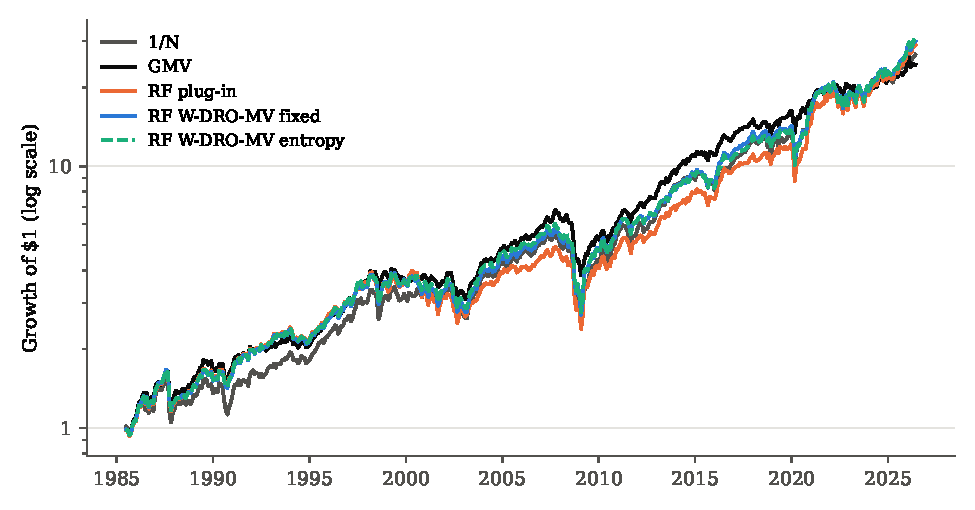
\includegraphics[width=0.95\linewidth]{fig_wealth.pdf}
\caption{Cumulative net excess wealth (10bp costs), July 1985--June 2026, log scale. Random-forest (RF) strategies use rolling validation of the radius.}\label{fig:wealth}
\end{figure}

\subsection{What the radius does}

Validation selects one radius per month, which can hide how the radius shapes the portfolio. Table~\ref{tab:grid} and Figure~\ref{fig:grid} therefore report every point on the grid. Two facts are clear.

\begin{figure}[!htbp]\centering
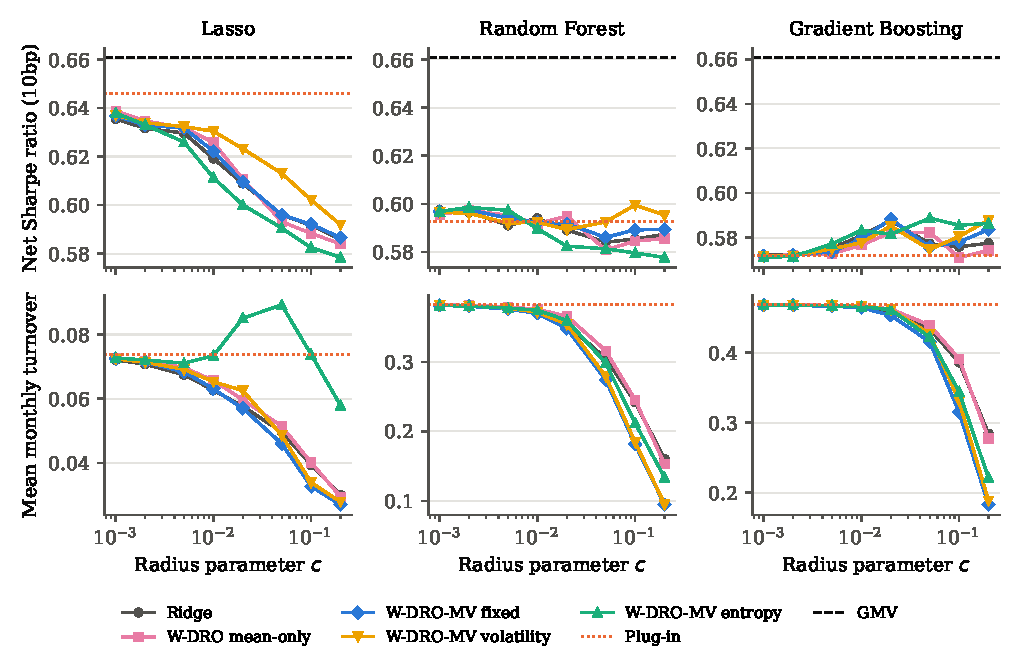
\includegraphics[width=\linewidth]{fig_grid.pdf}
\caption{Net Sharpe ratio (10bp, top row) and average monthly turnover (bottom row) against the radius parameter $c$, for each family and forecaster. Ridge uses $\lambda=3c$. Horizontal lines mark the plug-in portfolio (dotted) and GMV (dashed).}\label{fig:grid}
\end{figure}

\begin{table}[!htbp]\centering
\caption{The full radius grid: net Sharpe ratio (10bp) and turnover}\label{tab:grid}
\footnotesize\setlength{\tabcolsep}{4pt}\begin{tabular}{lrrrrrrrr}
\toprule
 & \multicolumn{8}{c}{Radius parameter $c$ (ridge: $\lambda = 3c$)} \\
\cmidrule(lr){2-9}
 & 0.001 & 0.002 & 0.005 & 0.01 & 0.02 & 0.05 & 0.1 & 0.2 \\
\midrule
\multicolumn{9}{l}{\textit{Lasso}} \\
\quad Ridge: net SR & 0.64 & 0.63 & 0.63 & 0.62 & 0.61 & 0.60 & 0.59 & 0.59 \\
\quad W-DRO mean-only: net SR & 0.64 & 0.63 & 0.63 & 0.63 & 0.61 & 0.59 & 0.59 & 0.58 \\
\quad W-DRO-MV fixed: net SR & 0.64 & 0.63 & 0.63 & 0.62 & 0.61 & 0.60 & 0.59 & 0.59 \\
\quad W-DRO-MV volatility: net SR & 0.64 & 0.63 & 0.63 & 0.63 & 0.62 & 0.61 & 0.60 & 0.59 \\
\quad W-DRO-MV entropy: net SR & 0.64 & 0.63 & 0.63 & 0.61 & 0.60 & 0.59 & 0.58 & 0.58 \\
\quad Ridge: turnover & 0.07 & 0.07 & 0.07 & 0.06 & 0.06 & 0.05 & 0.04 & 0.03 \\
\quad W-DRO-MV fixed: turnover & 0.07 & 0.07 & 0.07 & 0.06 & 0.06 & 0.05 & 0.03 & 0.03 \\
\quad W-DRO-MV entropy: turnover & 0.07 & 0.07 & 0.07 & 0.07 & 0.09 & 0.09 & 0.07 & 0.06 \\
\quad Plug-in: net SR 0.65, turnover 0.07 & \multicolumn{8}{l}{} \\
\addlinespace
\multicolumn{9}{l}{\textit{Random Forest}} \\
\quad Ridge: net SR & 0.60 & 0.60 & 0.59 & 0.59 & 0.59 & 0.58 & 0.59 & 0.59 \\
\quad W-DRO mean-only: net SR & 0.60 & 0.60 & 0.60 & 0.59 & 0.59 & 0.58 & 0.58 & 0.59 \\
\quad W-DRO-MV fixed: net SR & 0.60 & 0.60 & 0.59 & 0.59 & 0.59 & 0.59 & 0.59 & 0.59 \\
\quad W-DRO-MV volatility: net SR & 0.60 & 0.60 & 0.59 & 0.59 & 0.59 & 0.59 & 0.60 & 0.60 \\
\quad W-DRO-MV entropy: net SR & 0.60 & 0.60 & 0.60 & 0.59 & 0.58 & 0.58 & 0.58 & 0.58 \\
\quad Ridge: turnover & 0.38 & 0.38 & 0.38 & 0.37 & 0.35 & 0.30 & 0.24 & 0.16 \\
\quad W-DRO-MV fixed: turnover & 0.38 & 0.38 & 0.38 & 0.37 & 0.35 & 0.27 & 0.18 & 0.09 \\
\quad W-DRO-MV entropy: turnover & 0.38 & 0.38 & 0.38 & 0.37 & 0.36 & 0.30 & 0.21 & 0.13 \\
\quad Plug-in: net SR 0.59, turnover 0.38 & \multicolumn{8}{l}{} \\
\addlinespace
\multicolumn{9}{l}{\textit{Gradient Boosting}} \\
\quad Ridge: net SR & 0.57 & 0.57 & 0.58 & 0.58 & 0.59 & 0.58 & 0.58 & 0.58 \\
\quad W-DRO mean-only: net SR & 0.57 & 0.57 & 0.57 & 0.58 & 0.58 & 0.58 & 0.57 & 0.57 \\
\quad W-DRO-MV fixed: net SR & 0.57 & 0.57 & 0.57 & 0.58 & 0.59 & 0.58 & 0.58 & 0.58 \\
\quad W-DRO-MV volatility: net SR & 0.57 & 0.57 & 0.57 & 0.58 & 0.59 & 0.57 & 0.58 & 0.59 \\
\quad W-DRO-MV entropy: net SR & 0.57 & 0.57 & 0.58 & 0.58 & 0.58 & 0.59 & 0.59 & 0.59 \\
\quad Ridge: turnover & 0.47 & 0.47 & 0.47 & 0.47 & 0.46 & 0.43 & 0.39 & 0.28 \\
\quad W-DRO-MV fixed: turnover & 0.47 & 0.47 & 0.47 & 0.46 & 0.45 & 0.42 & 0.31 & 0.18 \\
\quad W-DRO-MV entropy: turnover & 0.47 & 0.47 & 0.47 & 0.47 & 0.46 & 0.42 & 0.34 & 0.22 \\
\quad Plug-in: net SR 0.57, turnover 0.47 & \multicolumn{8}{l}{} \\
\bottomrule
\end{tabular}
\begin{minipage}{0.97\linewidth}\footnotesize\smallskip
Each cell is a separate strategy with a fixed tuning parameter over the whole evaluation period (no validation). The volatility and entropy rules scale the radius as in \eqref{eq:radius}.
\end{minipage}
\end{table}

The Sharpe ratio is almost flat in the radius. For the random forest, the net Sharpe ratio of every family stays between 0.58 and 0.60 across a two-hundred-fold range of radii. For gradient boosting it stays between 0.57 and 0.59. For the Lasso it declines gently from 0.64 to about 0.58 as the portfolio moves from minimum-variance-like to $1/N$-like. There is no interior ``sweet spot'' to find, and no radius lifts any forecaster to the GMV benchmark.

Turnover, by contrast, falls steeply once the radius is large enough to bind. For the random forest, fixed-radius W-DRO-MV turnover falls from 0.38 to 0.09 at $c=0.2$ (a 75\% reduction), against 0.16 for ridge at the matched parameter. For gradient boosting it falls from 0.47 to 0.18, against 0.28 for ridge. The Wasserstein mean--variance penalty is thus a more turnover-efficient regulariser than ridge at equal Sharpe ratio. This is the one place where the distributional formulation differs materially from plain regularisation. Economically, robustness here acts as a trading-cost control device. It does not extract more value from the forecasts; it lets the investor hold them more cheaply.

\subsection{Regime uncertainty and forecast failure}

Does regime uncertainty tell us when forecasts fail? Figure~\ref{fig:entropy} plots $H_t$. Entropy is persistently high: its mean is 0.57. This is typical of monthly market returns, where the two regimes differ mainly in variance and a single month's return is weak evidence about the state. Its correlation with 12-month volatility is 0.31.

\begin{figure}[!htbp]\centering
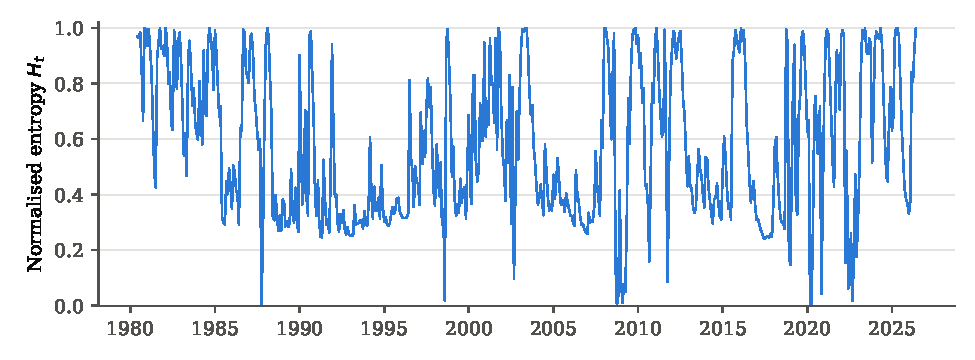
\includegraphics[width=0.95\linewidth]{fig_entropy.pdf}
\caption{Normalised entropy of filtered two-state HMM regime probabilities, June 1980--June 2026. Parameters are re-estimated each June on an expanding window using data up to the estimation date only.}\label{fig:entropy}
\end{figure}

Table~\ref{tab:mech} regresses monthly measures of forecast quality on standardised entropy, with and without a control for volatility. For the random forest and gradient boosting, a one-standard-deviation increase in entropy lowers the rank IC by 0.017 and 0.019 ($t=-1.82$ and $-2.16$). Adding volatility barely changes these estimates, and volatility itself does not predict the IC. The effect is large relative to the average IC of 0.007. Split by entropy terciles, the random-forest IC is 0.026 in low-entropy months and about zero in the other two terciles; the gradient-boosting IC is 0.028 and then about zero. The tree models carry cross-sectional information only when the regime is clear. Volatility predicts the mean absolute forecast error strongly ($t\approx4.4$ to $4.7$), but that is mechanical: large returns mean large errors. Entropy does not predict it. Neither variable predicts the return of a forecast-sorted long--short portfolio significantly, and the Lasso results, based on only 108 non-constant months, are uninformative.

\begin{table}[!htbp]\centering
\caption{Does regime uncertainty predict forecast quality?}\label{tab:mech}
\small\begin{tabular}{llrrrrr}
\toprule
Model & Dependent variable & $\beta_H$ & $t(\beta_H)$ & $\beta_{\sigma}$ & $t(\beta_{\sigma})$ & Months \\
\midrule
Lasso & Rank IC & $-$0.0009 & $-$0.04 &  &  & 108 \\
 & Rank IC & 0.0077 & 0.31 & $-$0.0340 & $-$1.51 & 108 \\
 & Long--short return & 0.0002 & 0.05 &  &  & 108 \\
 & Long--short return & 0.0022 & 0.56 & $-$0.0081 & $-$1.89 & 108 \\
 & Mean abs. error & $-$0.0022 & $-$0.77 &  &  & 108 \\
 & Mean abs. error & $-$0.0035 & $-$1.43 & 0.0050 & 1.58 & 108 \\
\midrule
Random Forest & Rank IC & $-$0.0174 & $-$1.82 &  &  & 492 \\
 & Rank IC & $-$0.0167 & $-$1.63 & $-$0.0024 & $-$0.19 & 492 \\
 & Long--short return & $-$0.0005 & $-$0.33 &  &  & 492 \\
 & Long--short return & $-$0.0005 & $-$0.24 & $-$0.0002 & $-$0.10 & 492 \\
 & Mean abs. error & 0.0012 & 0.68 &  &  & 492 \\
 & Mean abs. error & $-$0.0012 & $-$0.70 & 0.0076 & 4.36 & 492 \\
\midrule
Gradient Boosting & Rank IC & $-$0.0185 & $-$2.16 &  &  & 492 \\
 & Rank IC & $-$0.0197 & $-$2.14 & 0.0039 & 0.36 & 492 \\
 & Long--short return & $-$0.0012 & $-$0.82 &  &  & 492 \\
 & Long--short return & $-$0.0017 & $-$0.98 & 0.0016 & 0.86 & 492 \\
 & Mean abs. error & 0.0012 & 0.65 &  &  & 492 \\
 & Mean abs. error & $-$0.0015 & $-$0.83 & 0.0085 & 4.67 & 492 \\
\bottomrule
\end{tabular}
\begin{minipage}{0.95\linewidth}\footnotesize\smallskip
Monthly time-series regressions of forecast-quality measures for month $t+1$ on standardised regime entropy $H_t$ and standardised 12-month market volatility $\sigma_t$, both known at the end of month $t$. Rank IC is the Spearman correlation between forecasts and realised returns. Long--short return is the return of the top-10 minus bottom-10 industries sorted on the forecast. Newey--West $t$-statistics with six lags. Lasso regressions use months with a non-constant forecast only.
\end{minipage}
\end{table}

So the premise of the entropy rule holds, at least in direction. The question is whether it pays. It does not. In Table~\ref{tab:main}, the entropy-radius portfolios have net Sharpe ratios of 0.61, 0.60 and 0.59, against 0.60, 0.60 and 0.58 for the fixed radius. Table~\ref{tab:regime} splits performance by entropy and volatility terciles. The entropy-radius portfolio does not systematically outperform the fixed-radius portfolio in high-entropy months, where it is most conservative, or in low-entropy months, where it trusts the forecast most.

\begin{table}[!htbp]\centering
\caption{Net Sharpe ratio (10bp) by regime-uncertainty and volatility terciles}\label{tab:regime}
\small\begin{tabular}{lrrrrrr}
\toprule
 & \multicolumn{3}{c}{HMM entropy tercile} & \multicolumn{3}{c}{Volatility tercile} \\
\cmidrule(lr){2-4}\cmidrule(lr){5-7}
Strategy & Low & Mid & High & Low & Mid & High \\
\midrule
1/N & 0.47 & 0.65 & 0.61 & 0.92 & $-$0.08 & 1.14 \\
GMV & 0.40 & 0.86 & 0.74 & 1.10 & 0.05 & 1.11 \\
\midrule
Lasso, plug-in & 0.51 & 0.68 & 0.74 & 1.21 & 0.13 & 0.87 \\
Lasso, ridge & 0.45 & 0.73 & 0.62 & 1.07 & 0.09 & 0.91 \\
Lasso, fixed radius & 0.45 & 0.74 & 0.62 & 1.07 & 0.09 & 0.92 \\
Lasso, volatility radius & 0.46 & 0.70 & 0.66 & 1.09 & 0.07 & 0.93 \\
Lasso, entropy radius & 0.45 & 0.72 & 0.67 & 1.08 & 0.08 & 0.94 \\
\midrule
Random Forest, plug-in & 0.42 & 0.66 & 0.72 & 0.96 & 0.12 & 0.92 \\
Random Forest, ridge & 0.45 & 0.65 & 0.71 & 0.93 & 0.08 & 0.99 \\
Random Forest, fixed radius & 0.45 & 0.66 & 0.73 & 0.92 & 0.08 & 1.02 \\
Random Forest, volatility radius & 0.42 & 0.67 & 0.70 & 0.94 & 0.06 & 1.00 \\
Random Forest, entropy radius & 0.44 & 0.68 & 0.71 & 0.93 & 0.08 & 1.01 \\
\midrule
Gradient Boosting, plug-in & 0.47 & 0.58 & 0.67 & 0.99 & $-$0.03 & 1.02 \\
Gradient Boosting, ridge & 0.48 & 0.64 & 0.65 & 1.00 & $-$0.04 & 1.05 \\
Gradient Boosting, fixed radius & 0.49 & 0.64 & 0.64 & 1.02 & $-$0.02 & 1.03 \\
Gradient Boosting, volatility radius & 0.49 & 0.68 & 0.62 & 1.01 & $-$0.02 & 1.04 \\
Gradient Boosting, entropy radius & 0.49 & 0.64 & 0.64 & 1.03 & $-$0.05 & 1.04 \\
\bottomrule
\end{tabular}
\begin{minipage}{0.95\linewidth}\footnotesize\smallskip
Months are sorted into terciles of $H_t$ or of 12-month market volatility, measured at the decision date. Sharpe ratios are annualised within each tercile. Strategies use validated radii.
\end{minipage}
\end{table}

Two reasons explain the gap between prediction and profit. First, even in low-entropy months the forecasts are weak: an IC of about 0.03 is too small for a portfolio that trusts it to outperform a well-diversified minimum-variance portfolio after costs. Shrinking the radius when the regime is clear cannot create a signal that is not there. Second, a time-varying radius generates trading of its own. When $\varepsilon_t$ jumps, the optimal portfolio jumps with it, even if forecasts are unchanged. Figure~\ref{fig:grid} shows this clearly for the Lasso, where the entropy rule is the only family whose turnover \emph{rises} with the radius over part of the grid. For the tree models the effect is smaller but still visible: at $c=0.2$ the entropy rule turns over 0.13 and 0.22 per month, against 0.09 and 0.18 for the fixed radius.

\subsection{Statistical tests}

Table~\ref{tab:tests} collects bootstrap tests of the key Sharpe-ratio differences. None of the 30 tests that compare a robust rule with the plug-in portfolio, with ridge or with another radius rule is significant at 5\%. The only significant results concern the forecasts themselves: at 50bp the random-forest and gradient-boosting portfolios, plug-in or robust, underperform GMV by 0.15 to 0.22 in Sharpe ratio ($p\le0.014$), and the gradient-boosting plug-in portfolio also underperforms $1/N$ ($p=0.04$).

\begin{table}[!htbp]\centering
\caption{Bootstrap tests of Sharpe-ratio differences}\label{tab:tests}
\small\begin{tabular}{llrrrr}
\toprule
 & & \multicolumn{2}{c}{Net of 10bp} & \multicolumn{2}{c}{Net of 50bp} \\
\cmidrule(lr){3-4}\cmidrule(lr){5-6}
Model & Comparison (A minus B) & $\Delta$SR & $p$-value & $\Delta$SR & $p$-value \\
\midrule
Lasso & Plug-in $-$ GMV & $-$0.01 & 0.82 & $-$0.04 & 0.55 \\
 & Plug-in $-$ 1/N & 0.07 & 0.38 & 0.05 & 0.52 \\
 & W-DRO-MV fixed $-$ Plug-in & $-$0.04 & 0.34 & $-$0.05 & 0.24 \\
 & W-DRO mean-only $-$ Ridge & $-$0.00 & 0.21 & $-$0.00 & 0.23 \\
 & W-DRO-MV fixed $-$ Ridge & 0.00 & 0.82 & 0.00 & 0.84 \\
 & W-DRO-MV entropy $-$ W-DRO-MV fixed & 0.01 & 0.63 & 0.01 & 0.55 \\
 & W-DRO-MV entropy $-$ W-DRO-MV volatility & 0.01 & 0.71 & 0.01 & 0.64 \\
 & W-DRO-MV fixed $-$ GMV & $-$0.06 & 0.35 & $-$0.09 & 0.14 \\
\midrule
Random Forest & Plug-in $-$ GMV & $-$0.07 & 0.34 & $-$0.18 & 0.01 \\
 & Plug-in $-$ 1/N & 0.02 & 0.77 & $-$0.09 & 0.18 \\
 & W-DRO-MV fixed $-$ Plug-in & 0.01 & 0.78 & 0.03 & 0.36 \\
 & W-DRO mean-only $-$ Ridge & 0.00 & 0.93 & 0.00 & 0.93 \\
 & W-DRO-MV fixed $-$ Ridge & 0.01 & 0.54 & 0.01 & 0.14 \\
 & W-DRO-MV entropy $-$ W-DRO-MV fixed & $-$0.00 & 0.92 & $-$0.01 & 0.63 \\
 & W-DRO-MV entropy $-$ W-DRO-MV volatility & 0.01 & 0.34 & 0.01 & 0.38 \\
 & W-DRO-MV fixed $-$ GMV & $-$0.06 & 0.32 & $-$0.15 & 0.01 \\
\midrule
Gradient Boosting & Plug-in $-$ GMV & $-$0.09 & 0.24 & $-$0.22 & 0.01 \\
 & Plug-in $-$ 1/N & $-$0.00 & 0.97 & $-$0.12 & 0.04 \\
 & W-DRO-MV fixed $-$ Plug-in & 0.01 & 0.66 & 0.04 & 0.19 \\
 & W-DRO mean-only $-$ Ridge & $-$0.00 & 0.58 & $-$0.00 & 0.60 \\
 & W-DRO-MV fixed $-$ Ridge & $-$0.00 & 0.96 & 0.01 & 0.45 \\
 & W-DRO-MV entropy $-$ W-DRO-MV fixed & 0.00 & 0.89 & $-$0.00 & 0.90 \\
 & W-DRO-MV entropy $-$ W-DRO-MV volatility & $-$0.00 & 0.88 & $-$0.01 & 0.59 \\
 & W-DRO-MV fixed $-$ GMV & $-$0.08 & 0.26 & $-$0.18 & 0.01 \\
\midrule
None & GMV $-$ 1/N & 0.09 & 0.14 & 0.09 & 0.11 \\
None & Min CVaR $-$ 1/N & 0.05 & 0.44 & 0.04 & 0.57 \\
\bottomrule
\end{tabular}
\begin{minipage}{0.97\linewidth}\footnotesize\smallskip
$\Delta$SR is the difference in annualised net Sharpe ratios, strategy A minus strategy B. Two-sided $p$-values from the stationary bootstrap \citep{politis1994} with mean block length 6 and 3{,}000 resamples. Robust strategies use validated penalties or radii.
\end{minipage}
\end{table}

\section{Robustness and discussion}\label{sec:robust}

\paragraph{Risk aversion and subperiods.} Table~\ref{tab:robust} repeats the main comparison for $\gamma=2$ and $\gamma=10$ and for two subperiods of about 20 years each. The conclusions do not change. The ordering between plug-in, ridge and the three W-DRO-MV rules shifts by a few hundredths of Sharpe ratio from one specification to another, with no consistent winner. GMV is at or near the top in every specification. The one exception is the second half of the sample, where the Lasso plug-in portfolio, which is a minimum-variance portfolio in most months, edges ahead (0.69 against 0.66).

\begin{table}[!htbp]\centering
\caption{Robustness: risk aversion and subperiods}\label{tab:robust}
\footnotesize\setlength{\tabcolsep}{3.5pt}\begin{tabular}{lrrrrrrrrrr}
\toprule
 & \multicolumn{2}{c}{$\gamma=2$} & \multicolumn{2}{c}{$\gamma=5$} & \multicolumn{2}{c}{$\gamma=10$} & \multicolumn{2}{c}{1985--2005} & \multicolumn{2}{c}{2006--2026} \\
\cmidrule(lr){2-3}\cmidrule(lr){4-5}\cmidrule(lr){6-7}\cmidrule(lr){8-9}\cmidrule(lr){10-11}
Strategy & SR$_{10}$ & TO & SR$_{10}$ & TO & SR$_{10}$ & TO & SR$_{10}$ & TO & SR$_{10}$ & TO \\
\midrule
1/N & 0.57 & 0.03 & 0.57 & 0.03 & 0.57 & 0.03 & 0.56 & 0.03 & 0.59 & 0.03 \\
GMV & 0.66 & 0.01 & 0.66 & 0.01 & 0.66 & 0.01 & 0.66 & 0.01 & 0.66 & 0.00 \\
\midrule
Lasso, plug-in & 0.61 & 0.08 & 0.65 & 0.07 & 0.63 & 0.07 & 0.61 & 0.11 & 0.69 & 0.04 \\
Lasso, ridge & 0.58 & 0.08 & 0.60 & 0.11 & 0.63 & 0.11 & 0.58 & 0.12 & 0.62 & 0.10 \\
Lasso, fixed & 0.58 & 0.08 & 0.60 & 0.11 & 0.62 & 0.11 & 0.59 & 0.11 & 0.62 & 0.10 \\
Lasso, volatility & 0.60 & 0.08 & 0.61 & 0.11 & 0.62 & 0.10 & 0.57 & 0.11 & 0.65 & 0.10 \\
Lasso, entropy & 0.59 & 0.09 & 0.61 & 0.10 & 0.63 & 0.10 & 0.59 & 0.10 & 0.64 & 0.09 \\
\midrule
RF, plug-in & 0.57 & 0.41 & 0.59 & 0.38 & 0.60 & 0.34 & 0.54 & 0.44 & 0.64 & 0.32 \\
RF, ridge & 0.61 & 0.33 & 0.60 & 0.33 & 0.60 & 0.29 & 0.59 & 0.35 & 0.60 & 0.31 \\
RF, fixed & 0.60 & 0.31 & 0.60 & 0.30 & 0.59 & 0.25 & 0.60 & 0.31 & 0.61 & 0.29 \\
RF, volatility & 0.60 & 0.32 & 0.59 & 0.31 & 0.61 & 0.25 & 0.60 & 0.31 & 0.59 & 0.31 \\
RF, entropy & 0.60 & 0.31 & 0.60 & 0.32 & 0.59 & 0.27 & 0.62 & 0.33 & 0.59 & 0.31 \\
\midrule
GB, plug-in & 0.58 & 0.48 & 0.57 & 0.47 & 0.59 & 0.44 & 0.59 & 0.50 & 0.56 & 0.44 \\
GB, ridge & 0.56 & 0.40 & 0.59 & 0.40 & 0.59 & 0.39 & 0.59 & 0.44 & 0.59 & 0.36 \\
GB, fixed & 0.57 & 0.38 & 0.58 & 0.37 & 0.60 & 0.34 & 0.59 & 0.42 & 0.58 & 0.32 \\
GB, volatility & 0.56 & 0.39 & 0.59 & 0.36 & 0.59 & 0.34 & 0.60 & 0.41 & 0.58 & 0.31 \\
GB, entropy & 0.59 & 0.39 & 0.59 & 0.38 & 0.60 & 0.35 & 0.60 & 0.42 & 0.58 & 0.33 \\
\bottomrule
\end{tabular}
\begin{minipage}{0.97\linewidth}\footnotesize\smallskip
SR$_{10}$ is the annualised Sharpe ratio net of 10bp costs; TO is average monthly turnover. Subperiod results use $\gamma=5$. Robust strategies use validated penalties or radii.
\end{minipage}
\end{table}

\paragraph{Why the earlier evidence looked better.} An earlier version of this study reported large Sharpe gains from W-DRO. Those gains came from simulated returns and from selecting the best radius after seeing the results. They did not survive real data, identical constraints and radius selection without hindsight. The contrast is itself a finding: DRO results that depend on the radius chosen after the fact should be read with care, because the radius is precisely the parameter that the method leaves open.

\paragraph{Limitations.} The forecasting signals are deliberately simple and the assets are industry portfolios, where predictability is weaker than in the cross-section of individual stocks. With stronger signals, for example from firm characteristics \citep{gu2020}, robustness may have more to work with, and the entropy rule may help more. The regime model uses only the market return; richer state variables may identify regimes more sharply and lower average entropy. The radius rules use one scale parameter and a simple linear map from the signal; learning this map, as in \citet{guo2026a}, is a natural extension, though the smoothness of the radius should be controlled to avoid the turnover effect documented here. Finally, the analysis is single-period. A multi-period formulation could trade off the benefit of a new radius against the cost of moving to it.

\section{Conclusion}\label{sec:conc}

Wasserstein robustness is often presented as a way to make ML forecasts safe to use in portfolios. On 41 years of out-of-sample industry returns, with identical constraints and no hindsight in the choice of radius, I find that it does not raise risk-adjusted performance. It does not turn weak forecasts into strategies that beat a forecast-free minimum-variance portfolio. What it does, reliably, is reduce trading: large radii cut turnover by up to three-quarters at no measurable cost in Sharpe ratio. The popular mean-only formulation is simply ridge regularisation, while the full Wasserstein mean--variance formulation is a somewhat more turnover-efficient regulariser. Regime uncertainty identifies the months in which tree-based forecasts stop working, but tying the radius to it does not improve portfolios, both because the forecasts are too weak even in good months and because a moving radius creates its own trading.

The broader lesson is that robustness manages the \emph{cost} of acting on uncertain forecasts; it cannot supply the forecasting skill. Whether regime-aware robustness pays with stronger signals, richer regime models or explicitly multi-period rebalancing is left for future work.

\clearpage
\bibliographystyle{apalike}
\bibliography{refs}

\end{document}
